
\begin{frame}
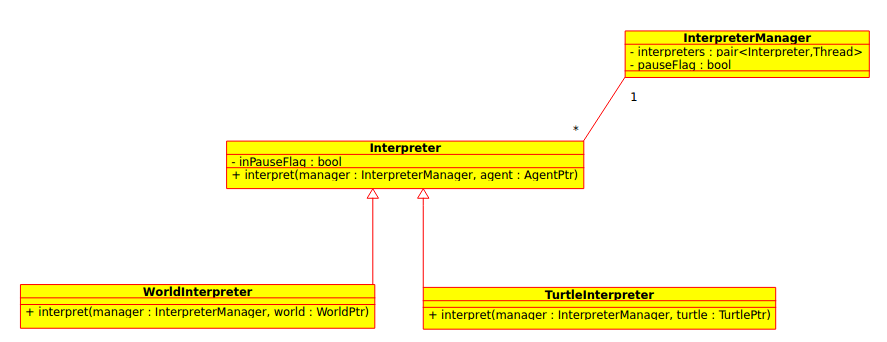
\includegraphics[scale=0.3]{doc/report/uml/interpreterUML.png}
\end{frame}

\begin{frame}
Rôle de l'interprète manager~:
\begin{itemize}
	\item Alerter des éventuelles pauses~;
	\item Création d'un monde avec les directives choisies~;
	\item Gérer les interpréteurs existants~;
	\item Stocker les couples threads-interprete créés.
\end{itemize}
C'est une sorte de gestionnaire d'interpréteurs.
\end{frame}

\begin{frame}
Reprenons notre arbre abstrait.
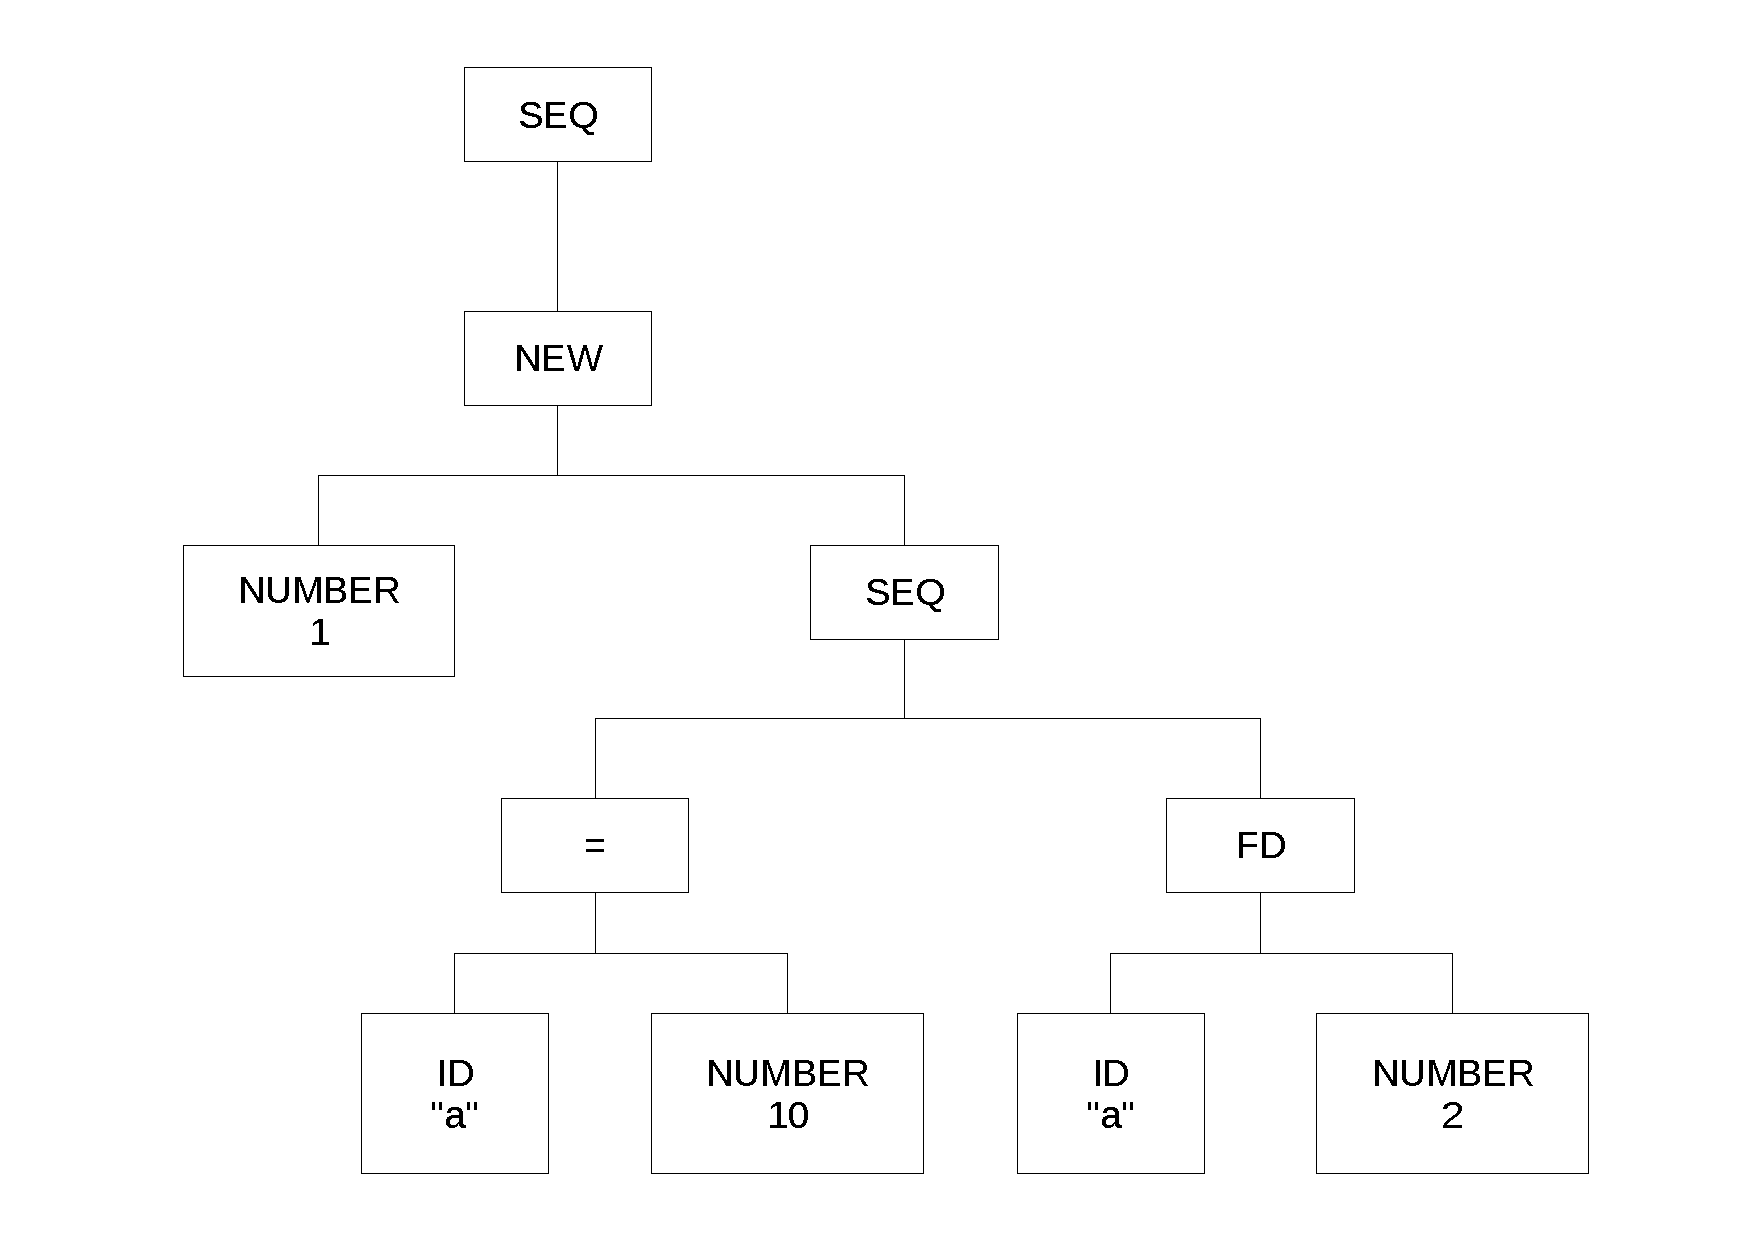
\includegraphics[scale=0.3]{doc/Presentation/img/arbre.pdf}
\note{L'interprete fonctionne de la manière suivante : lors de l'analyse d'un jeton, qui correspond à un nœud de l'arbre syntaxique, on analyse d'abord ses enfants (s'il y en a) puis ensuite le contenu du noeud courant.}
\end{frame}

\begin{frame}
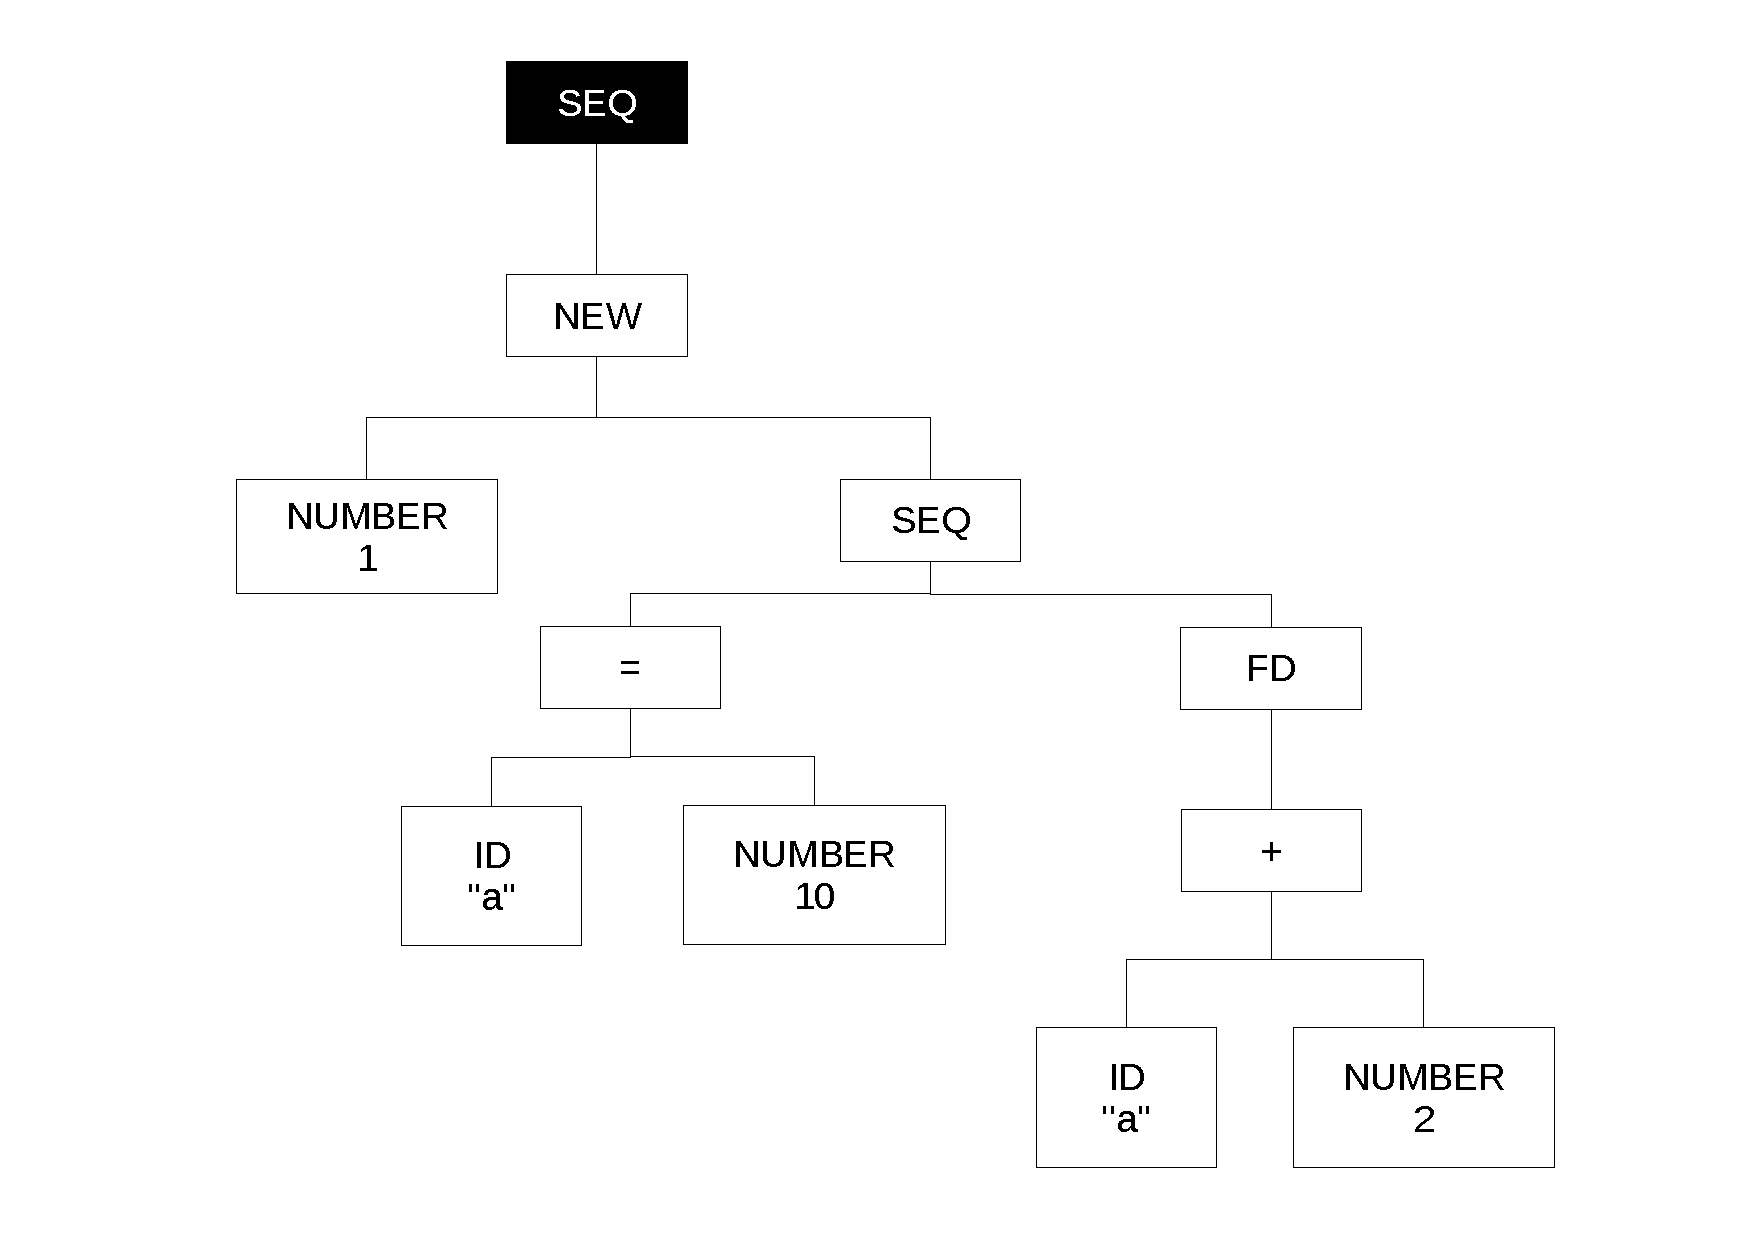
\includegraphics[scale=0.3]{doc/Presentation/img/arbre1.pdf}
\end{frame}

\begin{frame}
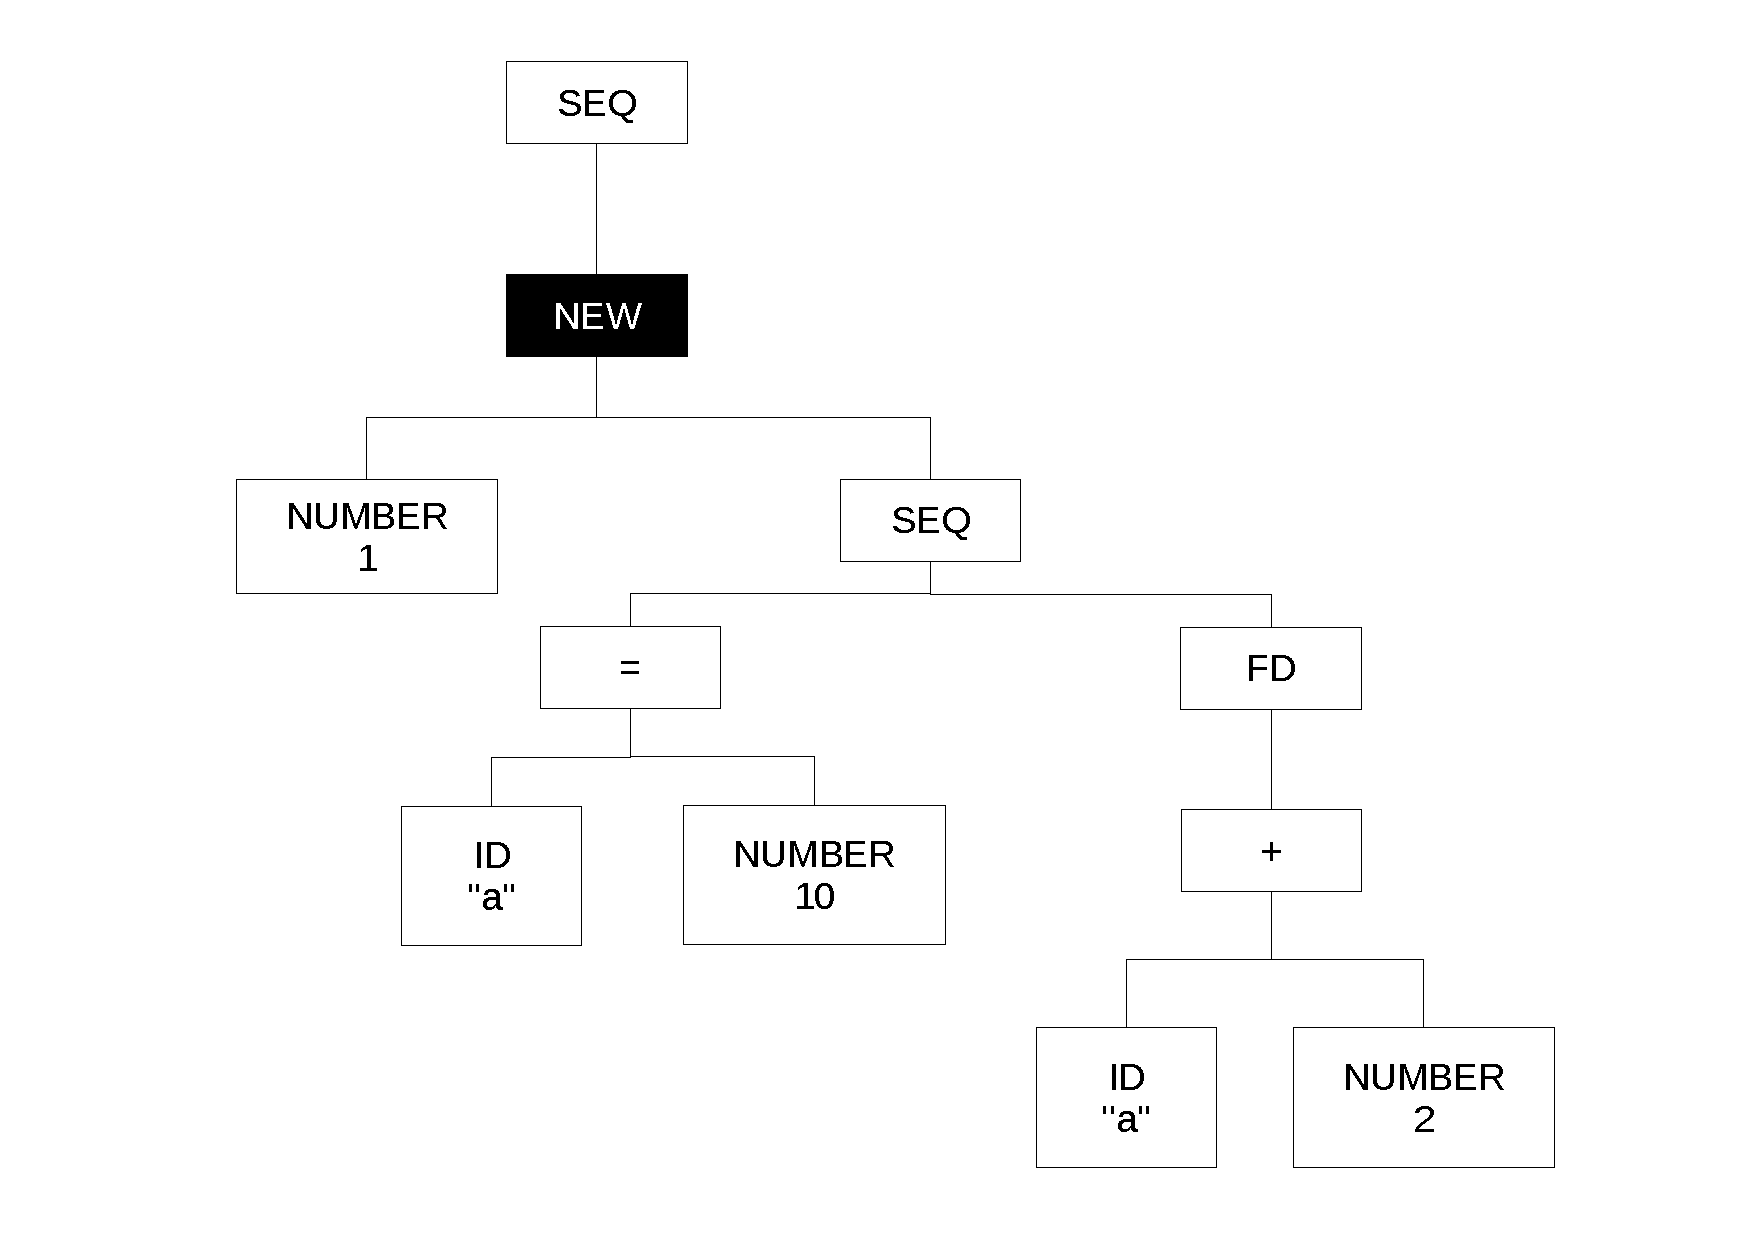
\includegraphics[scale=0.3]{doc/Presentation/img/arbre2.pdf}
\end{frame}

\begin{frame}
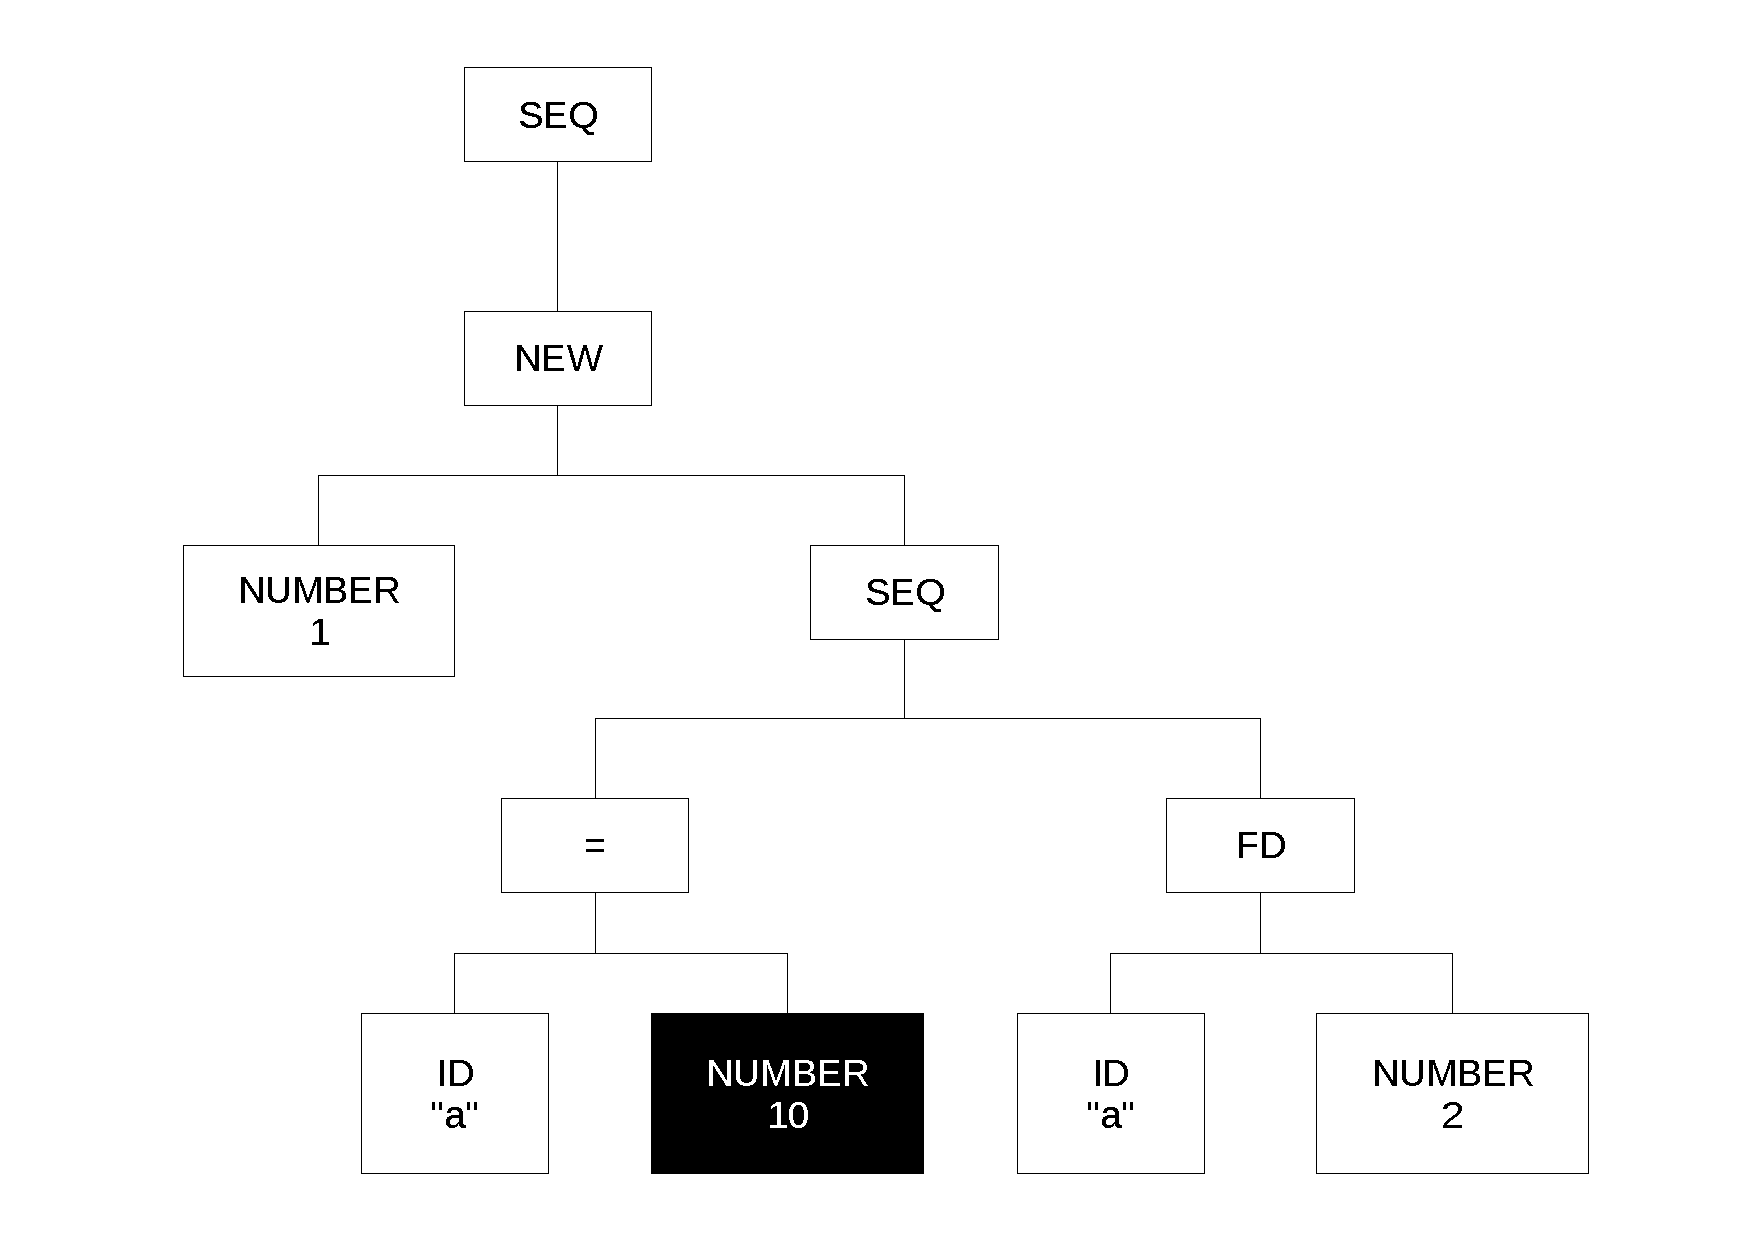
\includegraphics[scale=0.3]{doc/Presentation/img/arbre3.pdf}
\end{frame}

\begin{frame}
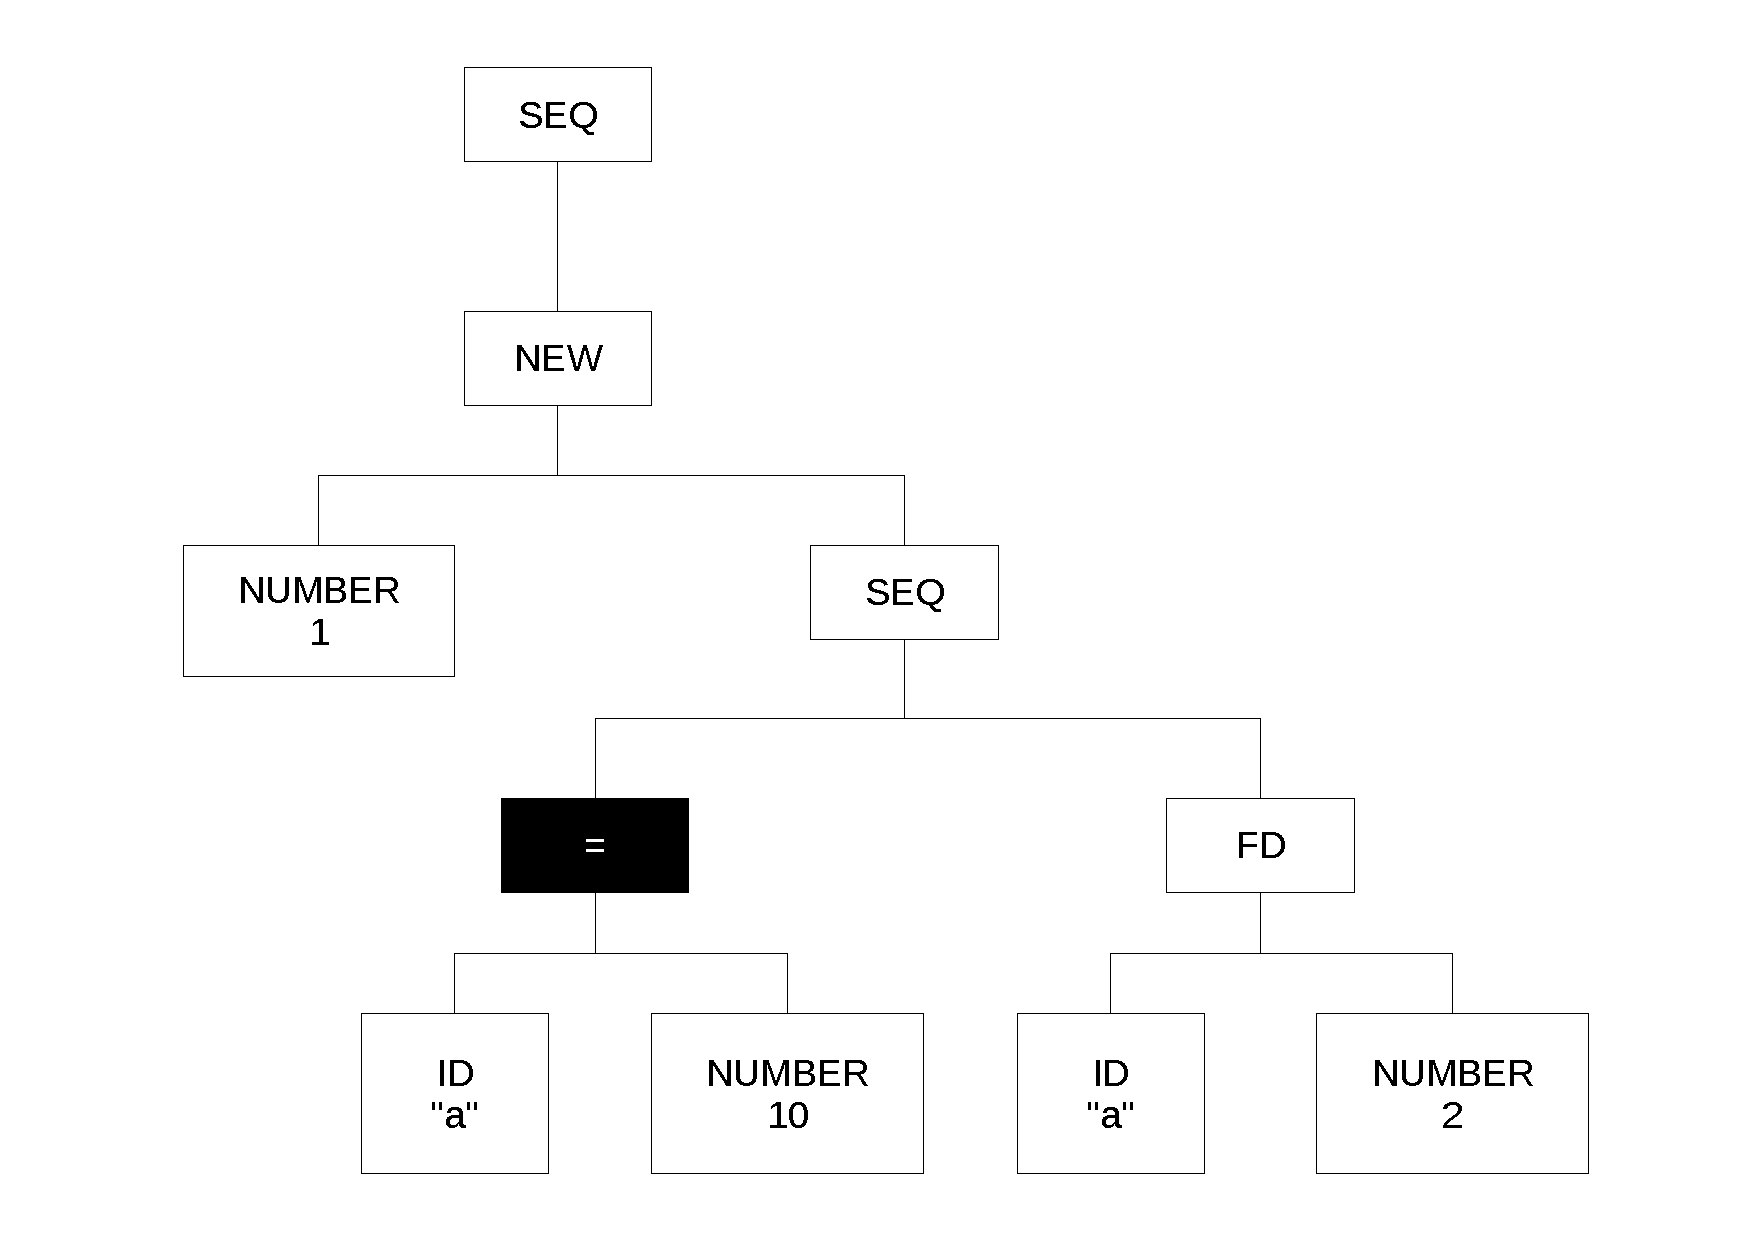
\includegraphics[scale=0.3]{doc/Presentation/img/arbre4.pdf}
\end{frame}

\begin{frame}
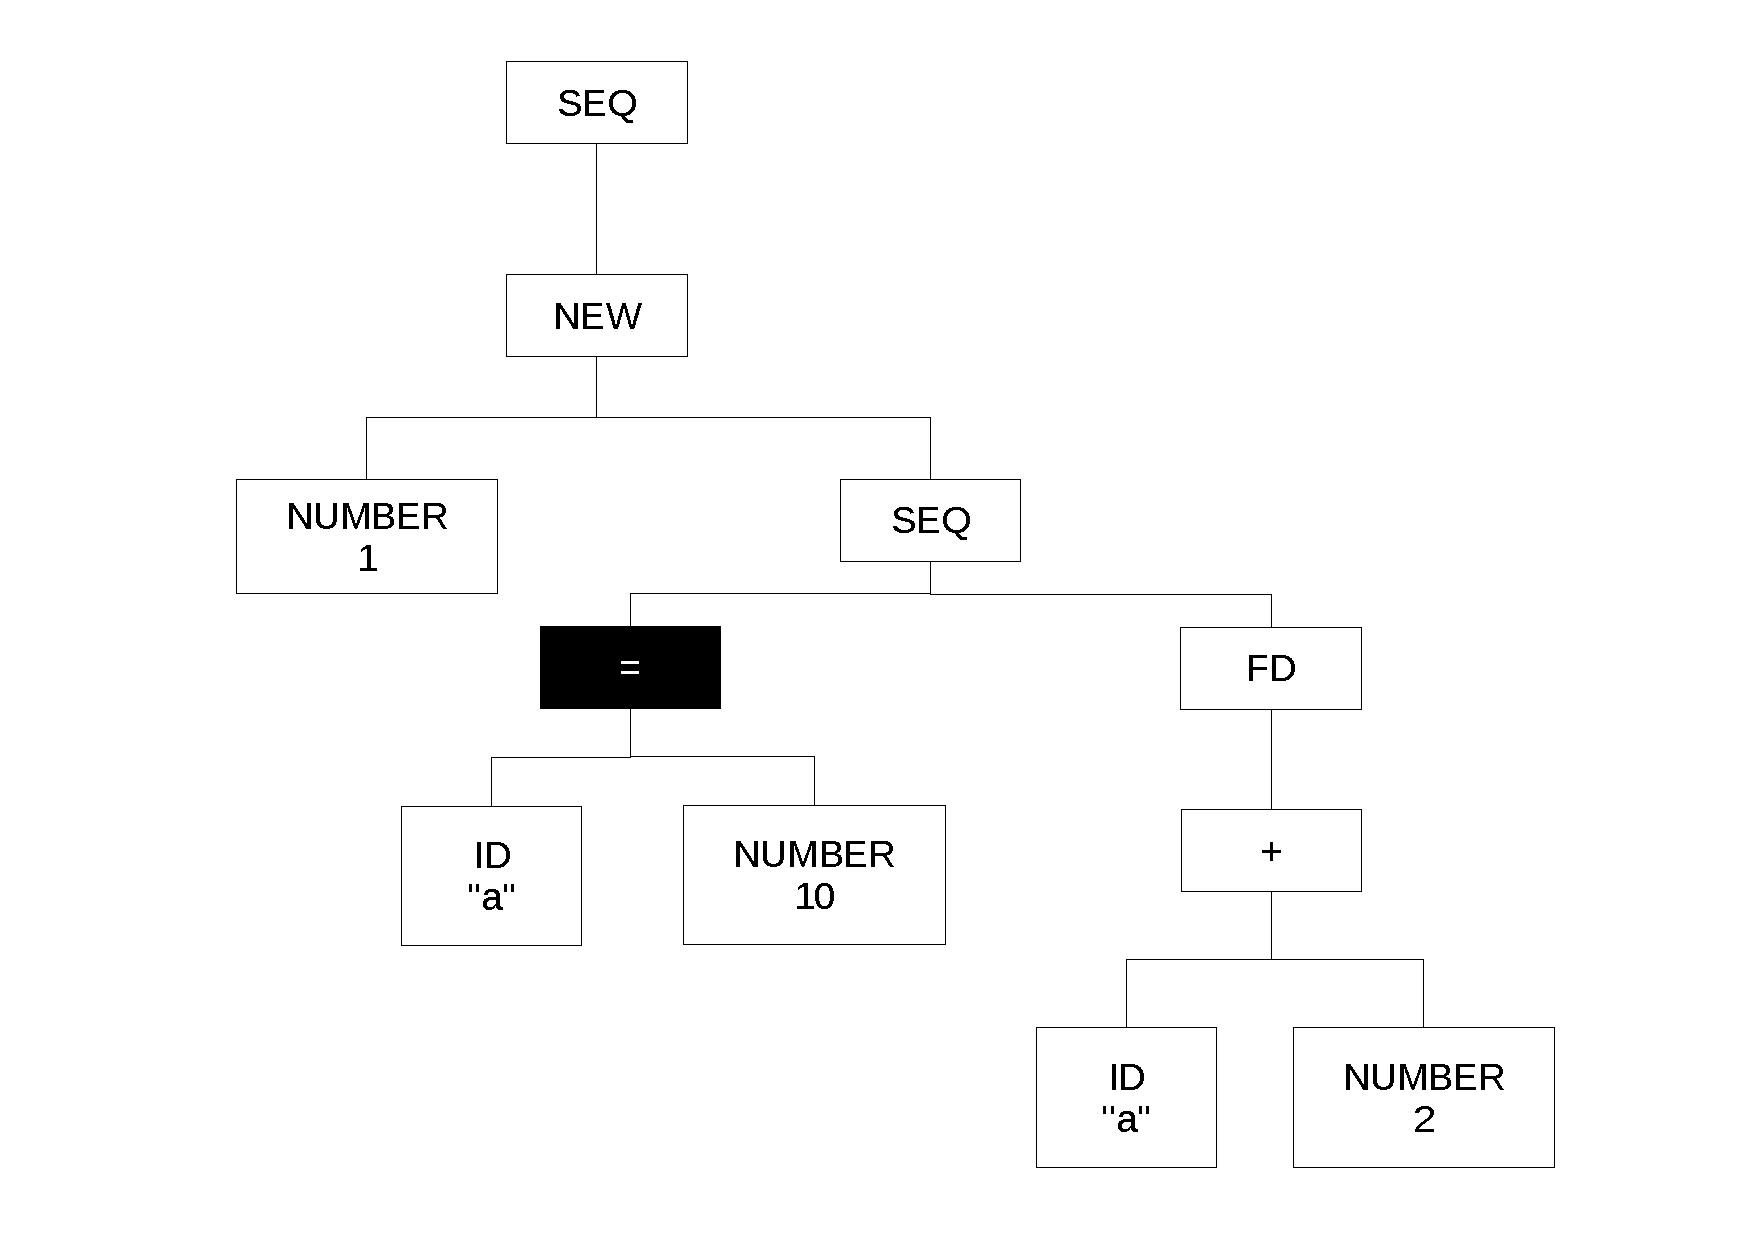
\includegraphics[scale=0.3]{doc/Presentation/img/arbre5.pdf}
\end{frame}

\begin{frame}
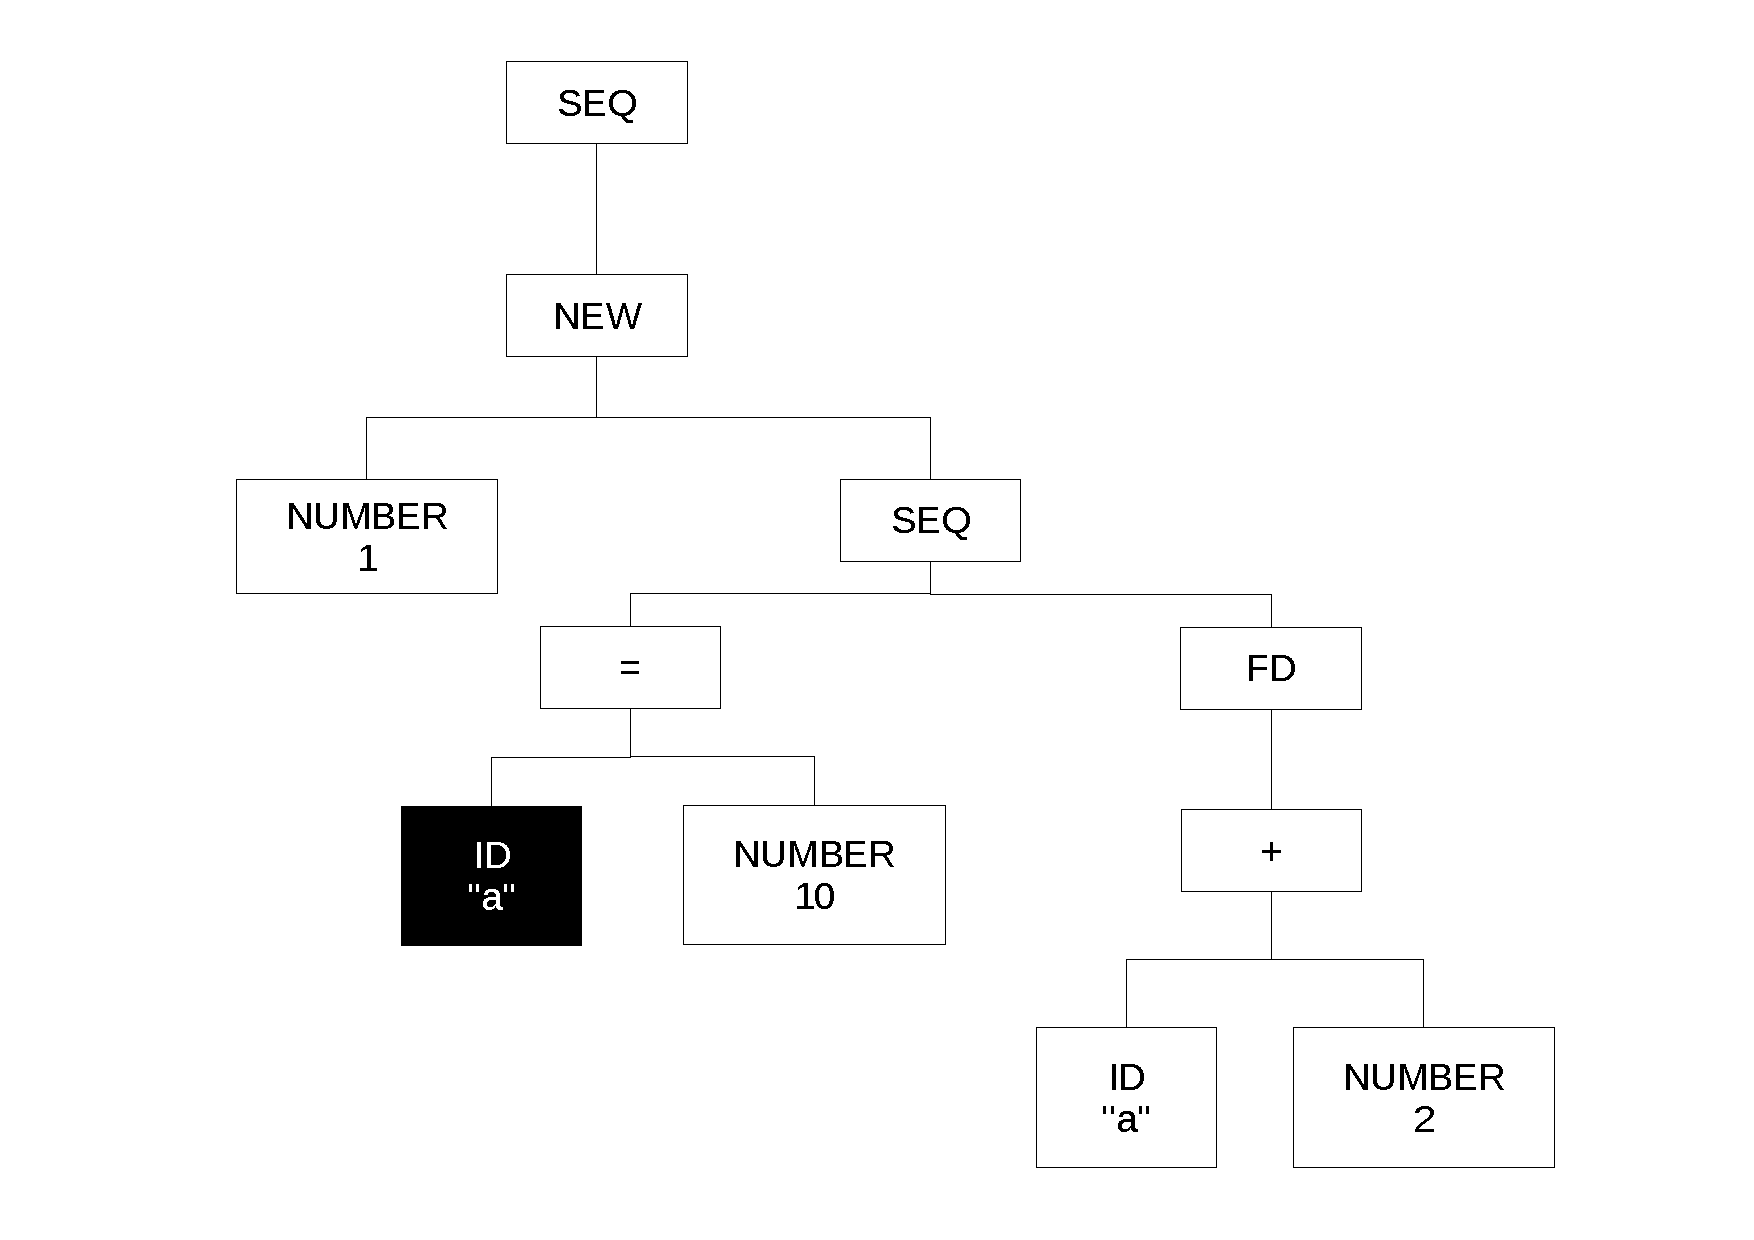
\includegraphics[scale=0.3]{doc/Presentation/img/arbre6.pdf}
\end{frame}

\begin{frame}
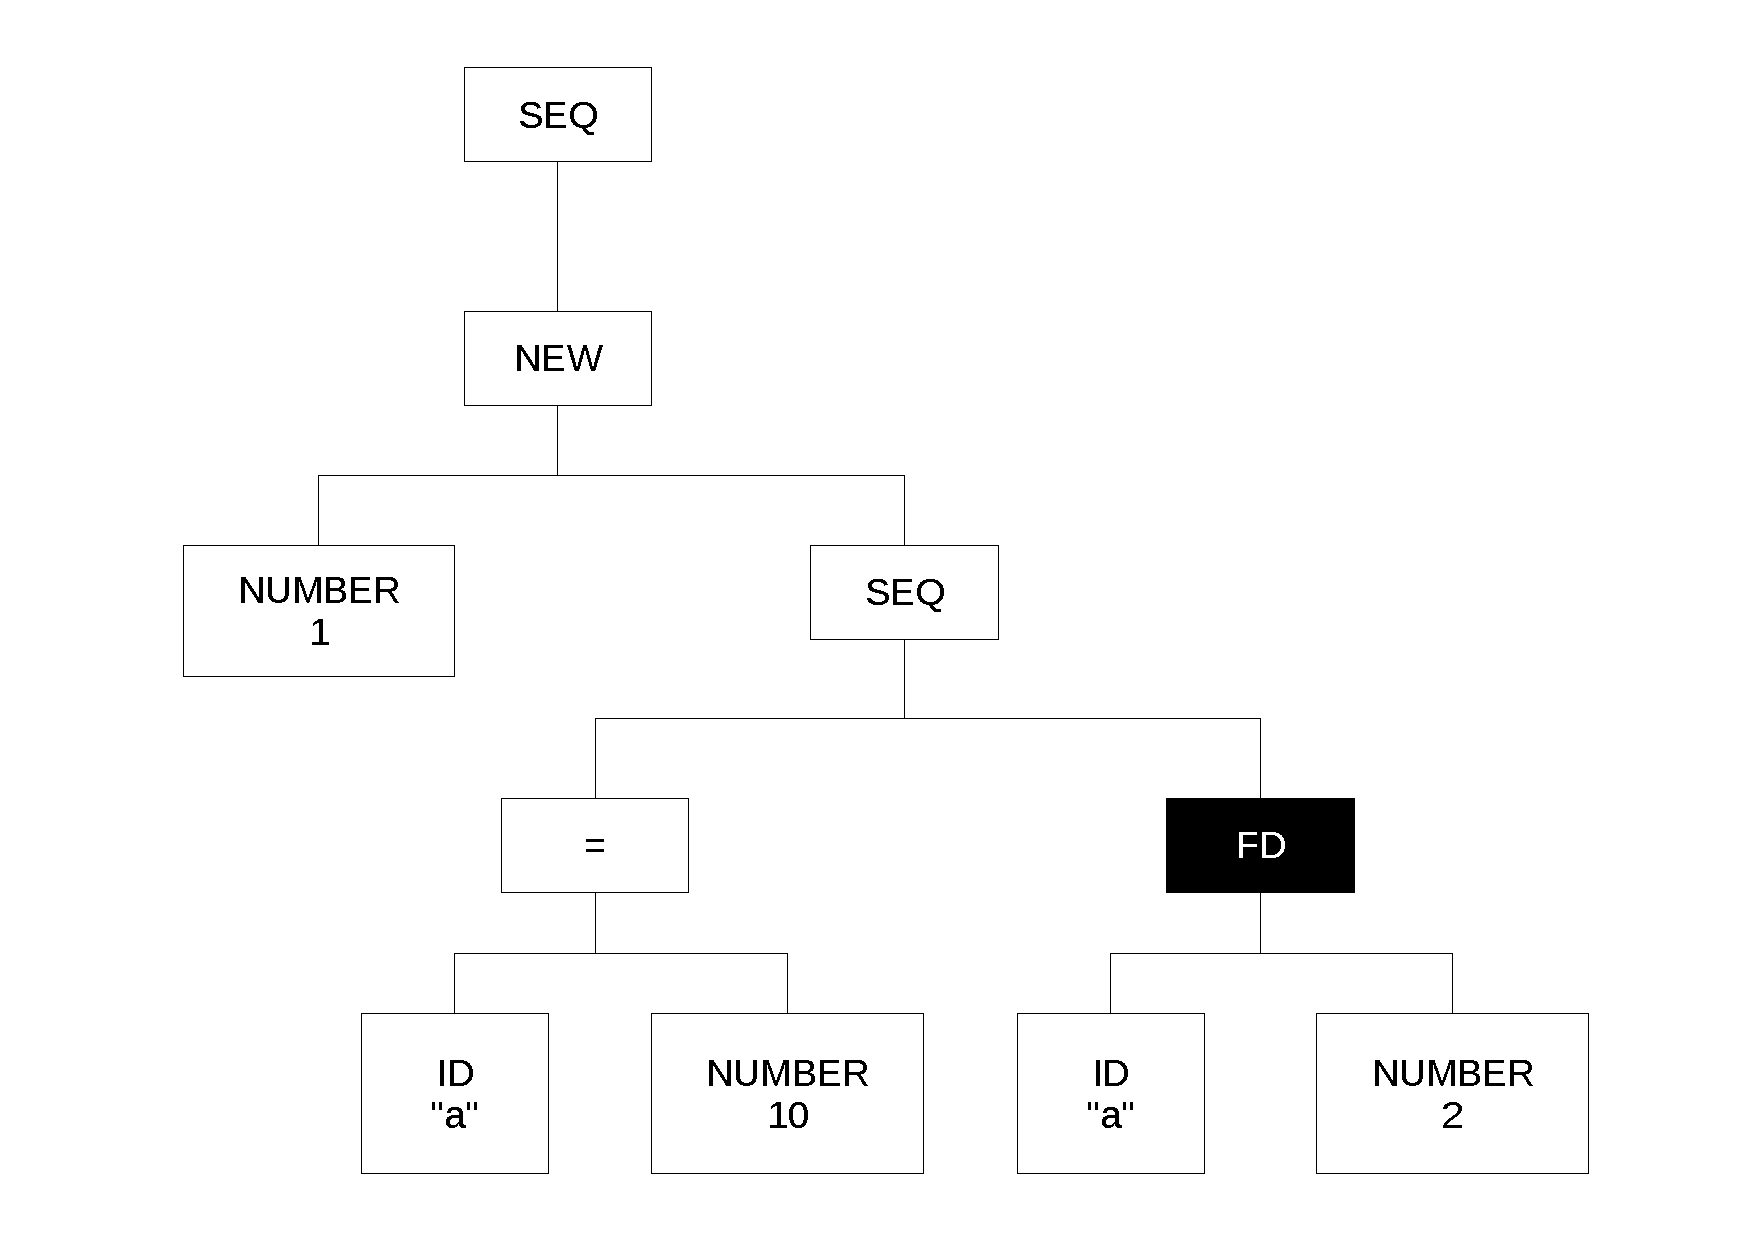
\includegraphics[scale=0.3]{doc/Presentation/img/arbre7.pdf}
\end{frame}

\begin{frame}
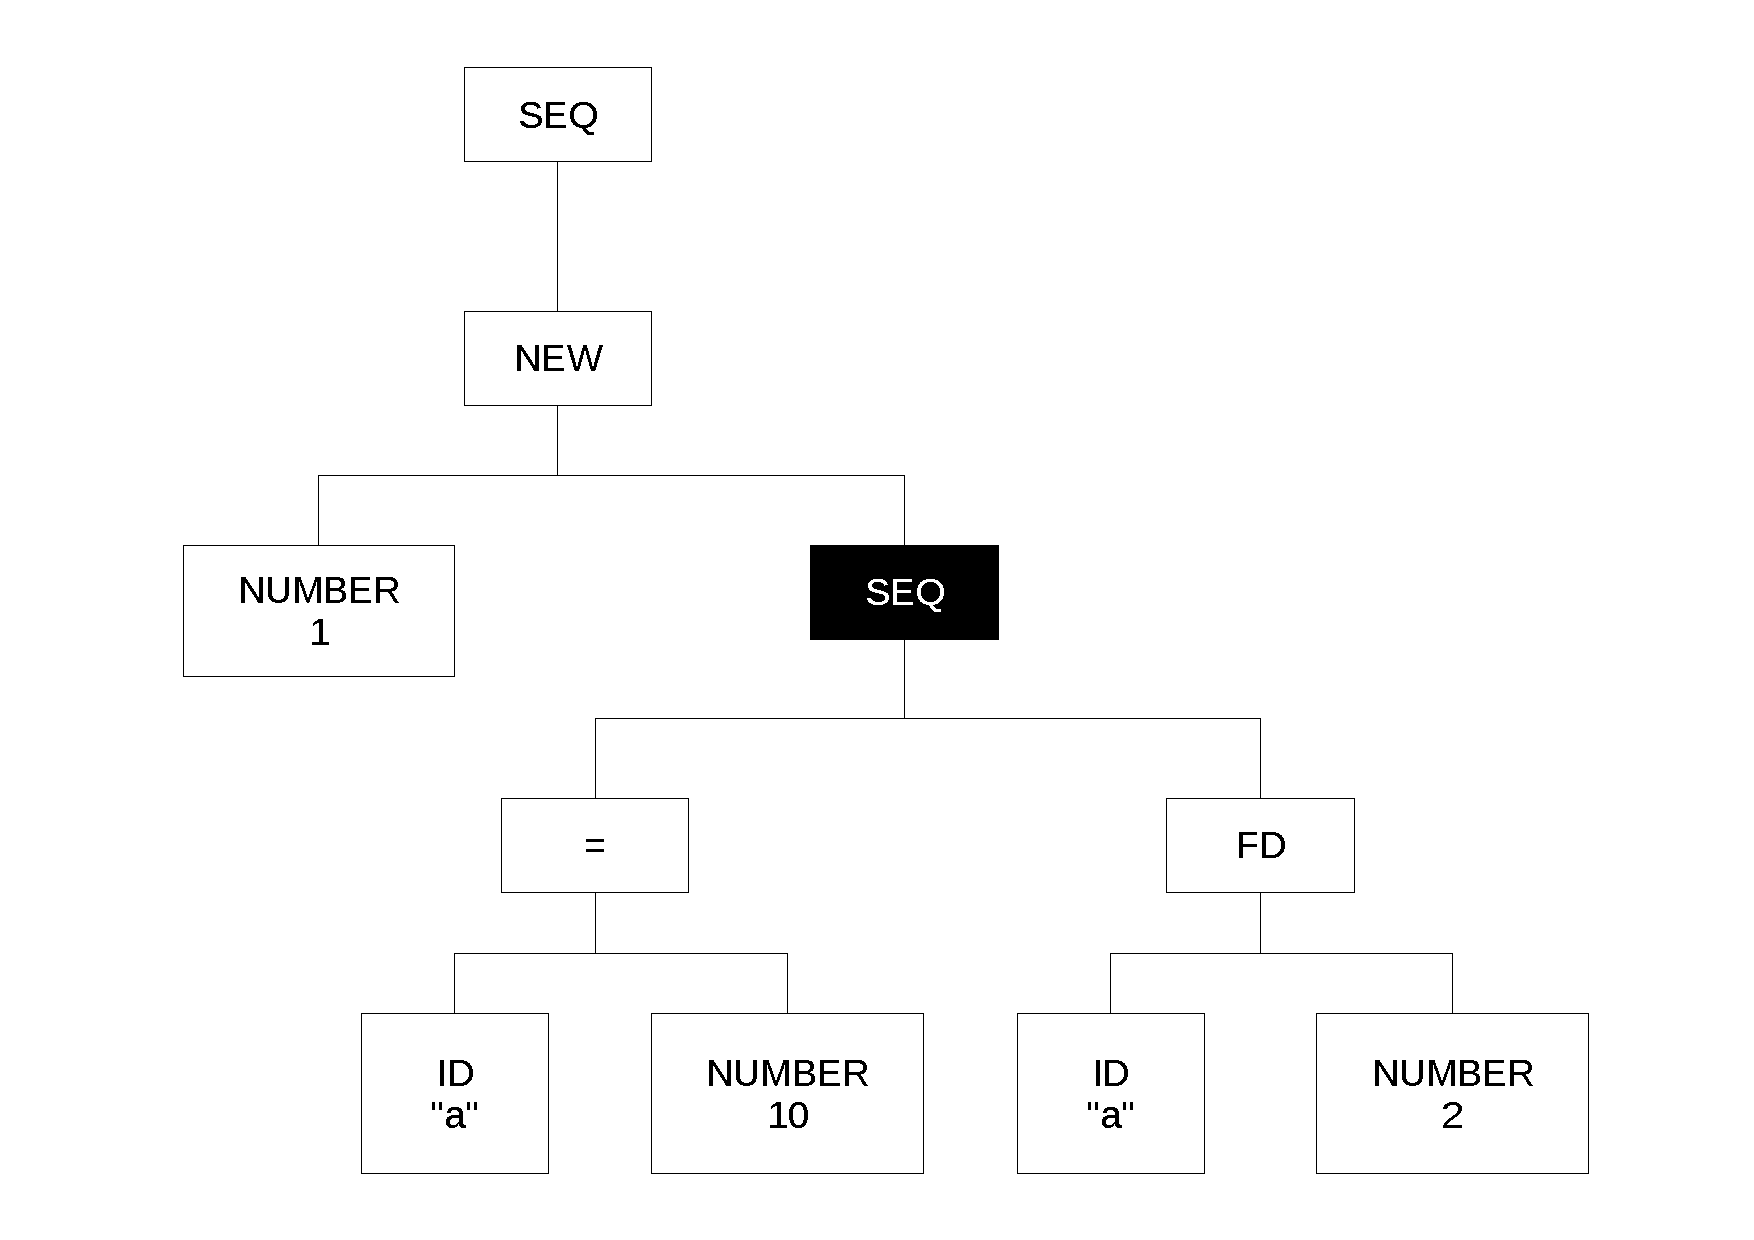
\includegraphics[scale=0.3]{doc/Presentation/img/arbre8.pdf}
\end{frame}

\begin{frame}
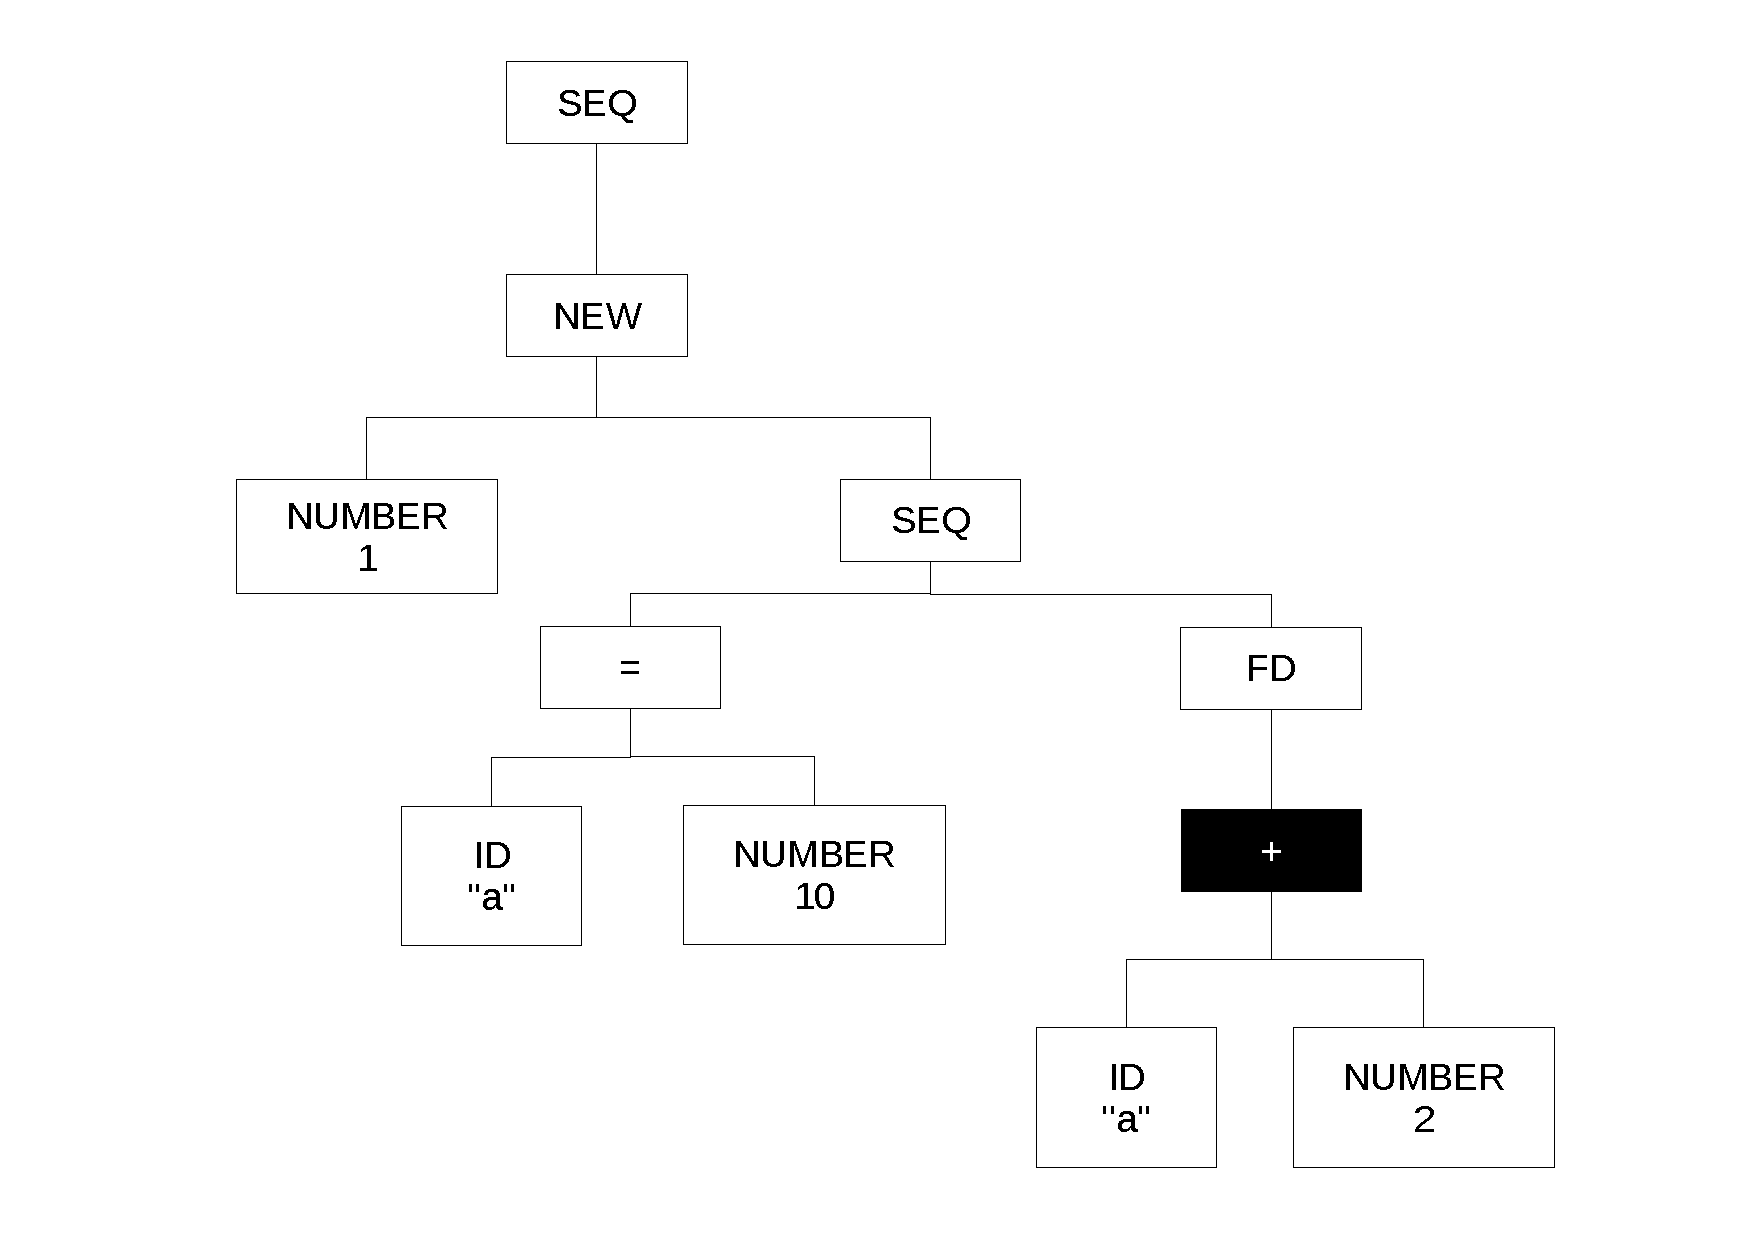
\includegraphics[scale=0.3]{doc/Presentation/img/arbre9.pdf}
\end{frame}

\begin{frame}
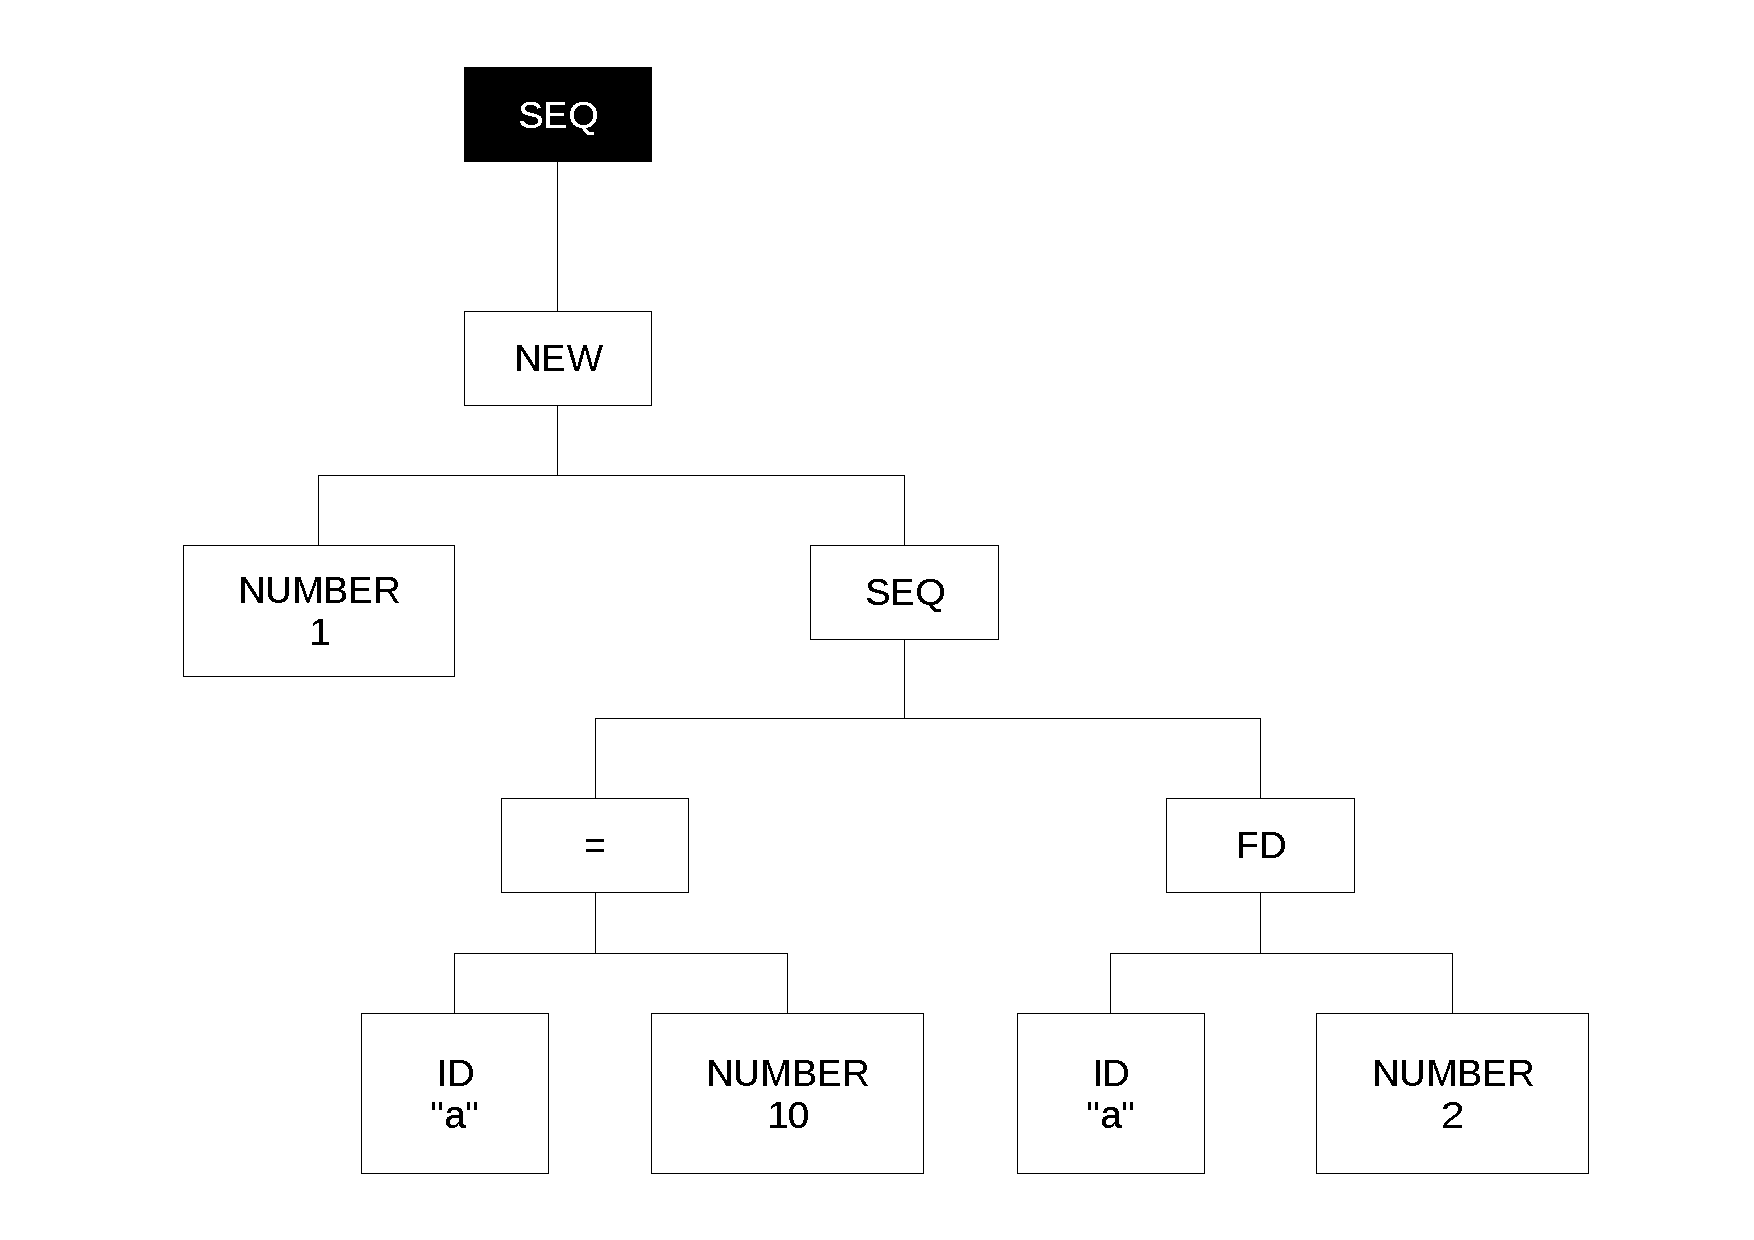
\includegraphics[scale=0.3]{doc/Presentation/img/arbre10.pdf}
\end{frame}

